% STATUS: verified
\chapter{Work products of a compliance programme}\label{ch:programme}

A compliance report says where a company stands against the law. A compliance management system
also needs documents of its own: a policy, an allocation of responsibilities, an assessment of
legal risk. The system drafts three such documents from the company's own library, holds each
draft to a fixed set of rules by code, and leaves the editing and the approval to a person.
This chapter describes what these documents are, how one is generated, what the six prompts
behind them ask, which rules the code enforces on the answers, how the numbers of the risk
register are computed, and what a person, the exports and the chat assistant can then do with a
draft. It ends with what a run costs and with the plain statement of how these prompts are, and
are not, measured.


% ------------------------------------------------------------
\section{What a work product is}\label{sec:programme:what}

A \term{work product} is one document of a company's compliance programme in one version: the
content the model drafted, the rules of its kind as that content met or broke them, a record
of what the run read, and what it cost. The application is \file{programme/} in the API; the
table is \code{work_products} (\cref{ch:data}). There are three \term{kinds}, and they are the
documents the second and third assignments of the course ask for (\cref{ch:course}).

\begin{table}[H]
\caption{The three kinds of work product (\file{programme/kinds.py}, \code{KINDS}); the title is the one the console prints}\label{tab:programme:kinds}
\begin{tabularx}{\textwidth}{@{}L{19mm}L{37mm}YL{17mm}@{}}
\toprule
\hd{Kind} & \hd{Title} & \hd{What it holds} & \hd{Builds on} \\
\midrule
\code{policy} & \lt{Atitikties politika} (Compliance policy) &
  The compliance policy in eight parts, each with the passages of the company's documents it
  rests on, its legal basis and the points left to the governing body; every document of the
  library placed on a level of the document hierarchy; the level~2 and level~3 documents the
  company still lacks. & --- \\
\code{governance} & \lt{Valdymo struktūra, atitikties procesas ir RACI} (Structure, compliance process and RACI) &
  The positions and units the documents name; the roles that are missing or cannot work as
  documented; a proposed structure as a tree; the compliance management process in steps; the
  RACI matrix that gives every step to roles of the structure. & \code{policy} \\
\code{risks} & \lt{Teisinės atitikties rizikos vertinimo kriterijai ir registras} (Legal compliance risk criteria and register) &
  The likelihood and impact criteria; the five bands of the 5×5 matrix with what each means
  for the company; the risk scenarios with their scores and treatment --- together the legal
  risk register. & \code{policy}, \code{governance} \\
\bottomrule
\end{tabularx}
\end{table}

A kind is a Python module with five names: \code{TITLE} (per language), \code{NEEDS} (the
kinds it builds on), \code{STEPS} (the names of its two model calls as job steps),
\code{generate(run)} and \code{validate(content, library, language, judge=None)}. The column
\code{kind} carries no database constraint, so a fourth kind would need a module, its prompts
and its page in the console, and no migration.

\paragraph{What a kind takes from the others.} \code{NEEDS} names the earlier kinds; the run
looks each one up as the company's approved version with the highest number, or, when none is
approved, its newest draft (\code{Run.__init__} in \file{programme/run.py}). A kind can be
generated without them: the prompt is then told that there is none. What is handed over is
narrow and exact (\cref{fig:programme:builds}). The governance prompts receive three parts of
the policy --- \code{mandate}, \code{roles} and \code{processes}, each cut to 1,800
characters --- with the policy's version and whether it is approved. The risk scenarios
prompt receives the names of the nodes of the governance structure whose kind is \code{unit}
or \code{function}. The policy is listed among what the register builds on and is recorded in
its \code{basis}, but its text is given to neither of the two risk prompts. Every kind also
reads the company's latest report whose status is \code{done}, whether or not it has been
signed off (\cref{sec:programme:report}).

\begin{figure}[H]
\centering
\begin{tikzpicture}[node distance=11mm and 10mm]
  \node[svc, text width=56mm] (policy) {\textbf{policy}\\ {\scriptsize eight parts · document hierarchy · missing documents}};
  \node[svc, text width=56mm, below=of policy] (gov) {\textbf{governance}\\ {\scriptsize positions and gaps · structure · process · RACI matrix}};
  \node[svc, text width=56mm, below=of gov] (risks) {\textbf{risks}\\ {\scriptsize criteria · appetite · scenarios (the register)}};
  \node[store, text width=27mm, left=of gov] (lib) {the company's profile and library};
  \node[data, text width=24mm, right=of gov] (report) {the latest finished report};
  \draw[flow] (policy) -- node[lbl, right=1mm] {its parts \emph{mandate}, \emph{roles}, \emph{processes}} (gov);
  \draw[flow] (gov) -- node[lbl, right=1mm] {the units and functions of its structure} (risks);
  \draw[flow] (lib.north) |- (policy.west);
  \draw[flow] (lib) -- (gov);
  \draw[flow] (lib.south) |- (risks.west);
  \draw[flow] (report.north) |- (policy.east);
  \draw[flow] (report) -- (gov);
  \draw[flow] (report.south) |- (risks.east);
\end{tikzpicture}
\caption{What each kind is generated from. The profile and every document go whole into both
calls of every kind. The report reaches each kind as a brief of its acts, counts and open
themes; the scenarios of the register also receive its gravest open findings.}\label{fig:programme:builds}
\end{figure}

\paragraph{The stored row.} A row of \code{work_products} belongs to a company and a kind and
has a \code{version} that counts up per company and kind (a unique constraint), a
\code{language} (\code{lt} or \code{en}) and a \code{status}: \code{queued}, \code{running},
\code{draft}, \code{approved}, \code{failed} or \code{cancelled}. Four JSON columns carry the
substance. \code{content} is the product itself, shaped by its kind. \code{checks} is the list
of the kind's rules as the content last met or broke them. \code{basis} names what the run
read: the report's id, the earlier products with their versions and statuses, and every
document with its title and SHA-256, so that a reader can tell what a draft rests on.
\code{stats} holds the tokens and the cost of the run and the prompt versions and models
behind it. The row also records who created, last edited and approved it, and when.

\begin{humanbox}{The system drafts and checks; a person approves}
No code path sets a work product to \code{approved} except a signed-in user's approval request
(\code{product_item} in \file{programme/api/views.py}), which the product's page sends. A
product stays a draft for as long as nobody approves it. The PDF of a draft says so on its
cover --- \enquote{Draft --- not yet approved by a person} --- and the Word file under its
title; the Excel workbook carries no such mark.
\end{humanbox}


% ------------------------------------------------------------
\section{How a product is made}\label{sec:programme:generation}

A product is generated by one background job, \code{programme.generate}, in four steps: the
documents are read, the model is called twice, and the references of the answer are checked.
This section follows a run from the request to the draft.

\subsection{Starting a run}

A user starts a run on the company's \ui{Programa} (Programme) tab with \ui{Generuoti}
(Generate), after a dialog that states the duration and the cost and takes the document's
language; the chat assistant can start one too (\cref{sec:programme:chat}). Both send
\route{POST}{/api/companies/{id}/programme} with a kind and a language. The view
\code{company_programme} in \file{programme/api/views.py} answers 400 \code{INVALID_FIELD} to
an unknown kind or a language other than \code{lt} and \code{en}, and otherwise refuses the
request in three cases:

\begin{itemize}
  \item the company has no document with extracted text (409 \code{NO_DOCUMENTS}) --- a
        product is written from the library and from nothing else;
  \item the user has less than \code{MIN_BUDGET_TO_START_USD}~=~\$0.25 of today's budget
        left (429 \code{BUDGET_EXCEEDED}); a user without a daily limit always passes;
  \item a product of the same kind is already queued or running for the company (409
        \code{ALREADY_RUNNING}); the check and the insert run under a row lock on the
        company, so two simultaneous requests cannot both pass.
\end{itemize}

Otherwise it creates the row with the next version number and the status \code{queued},
enqueues the job with the payload \code{{product_id}}, and writes the audit entry
\code{programme.create}. Starting a new version never touches the earlier ones.

\subsection{The four steps and their progress}

The job handler is \code{generate} in \file{programme/run.py}. It builds a \code{Run} --- the
object a kind's module works with --- and runs the steps of \cref{tab:programme:steps}. Each
step opens a job step (\cref{ch:arch}) and writes onto the job the step's name and how far
through the run that step begins, from the constant \code{STARTS = (0, 5, 50, 92)}. The two
model calls are nearly all of a run's time, which is why they span the range from 5 to 92 per
cent. The product's page polls the product every three seconds while it is queued or running
and shows these four steps with a progress bar and the elapsed time, and --- to the user who
started the run, since a user sees only the jobs they started --- the duration of each finished
step and the cost so far (\file{pages/Programme/ProductProgress.jsx} in the console).

\begin{table}[H]
\caption{The steps of \code{programme.generate}, by kind}\label{tab:programme:steps}
\begin{tabularx}{\textwidth}{@{}rL{22mm}L{24mm}L{22mm}Y@{}}
\toprule
\hd{From} & \hd{policy} & \hd{governance} & \hd{risks} & \hd{What happens} \\
\midrule
0\,\%  & \code{documents} & \code{documents} & \code{documents} & The inventory of every document is read; the block shared by both calls is built. \\
5\,\%  & \code{policy} & \code{structure} & \code{criteria} & The first model call. \\
50\,\% & \code{document_gaps} & \code{process_raci} & \code{scenarios} & The second model call, given what the first wrote. \\
92\,\% & \code{references} & \code{references} & \code{references} & \code{validate}: the stored shape, the computed numbers, the quotes, the provisions, the rules. \\
\bottomrule
\end{tabularx}
\end{table}

\subsection{The library block}\label{sec:programme:library}

A work product is written from whole documents. \code{Run.prepare} first makes sure every
document has an \term{inventory} --- the structured reading of one document that the report
also uses (\cref{ch:company}). Inventories are cached per document; a document whose cached
inventory is missing or no longer current is read now, four documents at a time (\code{WORKERS = 4}), by the prompt
\prompt{report.inventory}, and that call belongs to this job and to its cost. The run then
builds one text that both model calls receive unchanged:

\begin{codefile}{The shared block, in outline (\code{Run.prepare})}
COMPANY
the profile in its compact form: the company's facts, its credentials, the standards it
adopted, its roles, and the list of documents [D1], [D2] … with title, type and summary

DOCUMENTS
<document ref="D1" title="…" kind="…">
the whole text of the document
</document>

<document ref="D2" title="…" kind="…">
…
\end{codefile}

The profile is rendered by \code{render_profile(compact=True)} and the documents by
\code{document_pack}, both in \file{analysis/pipeline.py}: the functions the gap analysis of
a report uses (\cref{ch:report}). The documents are numbered in the order of their upload, and
the refs \code{D1}, \code{D2}, … are how the model names a document in its answer.

\begin{codebox}{The limit: no product from excerpts}
\code{document_pack} answers nothing when the texts of the company's documents together
exceed \code{DOCUMENT_PACK_CHARS = 600_000} characters. A report then falls back to the
documents nearest to each batch of obligations. A work product does not: \code{Run.prepare}
raises, the product ends as \code{failed}, and its error reads \enquote{The company's
documents are too many to read whole --- work products are not generated from excerpts.} A
policy written from fragments of a library would state things the unread remainder
contradicts, and no rule of the kind could detect it.
\end{codebox}

The block travels as the call's \code{shared} argument, apart from the data that differs
between the two calls. The assistant service places it where the gateway's provider caches
it, so the second call of a run reads the library from the cache instead of paying for it
again; the mechanism and its measurement are in \cref{ch:models}. The library of the sample
company \demo{} is 26~documents and 261,000 characters, about 59,000 tokens in a gap-analysis
call (\file{docs/markdown/en/architecture.md}, measured on 10--11 November 2026).

\subsection{Two model calls, the second given the first}

Each kind asks the model twice, with \code{Run.ask}: one call to \code{run_prompt}
(\cref{ch:models}) with the prompt's slug, the kind's own data, the shared block, the JSON
schema of the answer, and three variables --- \code{LANGUAGE} (Lithuanian or English, from the
product's language), \code{TODAY} and \code{COMPANY_NAME}. The call is filed under its job
step and recorded against the user who started the job. Before each call the run checks
whether the job was cancelled.

The split into two calls follows the dependencies inside each document. The missing documents
are those the drafted policy needs in order to work, so the second policy call is told what
the first wrote. A RACI matrix may only name roles of the structure, so the second governance
call receives the nodes the first proposed, by id. Scenarios are scored against criteria, so
the second risk call receives the criteria the first worded. In all three kinds the second
call sees the first answer as the model gave it, before \code{validate} has brought it into
its stored shape.

\subsection{What the latest report contributes}\label{sec:programme:report}

The report enters a run as text built by code, not as findings the model may browse.
\code{report_brief} in \file{programme/policy.py} writes a short account of the company's
latest finished report: the acts it assessed (an upcoming act marked \enquote{applies
later}), the numbers of findings \status{met}, \status{partial}, \status{missing} and
\status{unknown} --- a reviewer's override counted in place of the model's status --- and, under \enquote{OPEN THEMES}, every category that has findings which
are \status{missing}, \status{unknown} or \status{partial}, largest first, with its counts and
a few of those findings by title, act and provision. The policy calls get four examples a
theme, the governance calls two, the criteria call one. The scenarios call gets a different
list instead, \code{_open_findings} in \file{programme/risks.py}: up to 36 open findings,
the gravest first by severity and then by status, each with its act, provision, obligation
title and the first 220 characters of its analysis. A company without a finished report is
described to the model as having none; the run goes on.

\begin{figure}[H]
\centering
\begin{tikzpicture}[node distance=4.5mm and 11mm]
  \node[man, text width=72mm] (user) {\textbf{A user asks for a kind}\\ {\scriptsize on the company's Programme tab, or in the chat after the user's yes}};
  \node[chk, text width=72mm, below=of user] (route) {\textbf{The API accepts or refuses}\\ {\scriptsize refused: no readable document · under \$0.25 of today's budget · one of this kind already in work}};
  \node[svc, text width=72mm, below=9mm of route] (docs) {\textbf{documents} · from 0\,\%\\ {\scriptsize every document's inventory · the shared block · stops when the library exceeds 600,000 characters}};
  \node[ai, text width=72mm, below=of docs] (c1) {\textbf{first call} · from 5\,\%\\ {\scriptsize the policy · the structure · the criteria}};
  \node[ai, text width=72mm, below=of c1] (c2) {\textbf{second call} · from 50\,\%\\ {\scriptsize hierarchy and missing documents · process and RACI · scenarios --- given what the first wrote}};
  \node[chk, text width=72mm, below=of c2] (refs) {\textbf{references} · from 92\,\%\\ {\scriptsize \code{validate}: stored shape · numbers computed · quotes located · provisions looked up · rules checked}};
  \node[svc, text width=72mm, below=9mm of refs] (draft) {\textbf{A draft}\\ {\scriptsize content · checks · basis · stats --- waiting for a person}};
  \node[ai, text width=37mm, right=of docs] (inv) {\textbf{inventory}\\ {\scriptsize only for a document not read before}};
  \coordinate (mid) at ($(c1.east)!.5!(c2.east)$);
  \node[data, text width=31mm, right=13mm of mid] (shared) {shared block\\ {\scriptsize the same text in both calls}};
  \node[ai, text width=37mm, right=of refs] (judge) {\textbf{citation judge}\\ {\scriptsize once: does each provision regulate what is said of it}};
  \draw[flow] (user) -- (route);
  \draw[flow] (route) -- (docs);
  \draw[flow] (docs) -- (c1);
  \draw[flow] (c1) -- (c2);
  \draw[flow] (c2) -- (refs);
  \draw[flow] (refs) -- (draft);
  \draw[opt] (docs) -- (inv);
  \draw[call] (shared.north west) -- (c1.east);
  \draw[call] (shared.south west) -- (c2.east);
  \draw[call] (refs) -- (judge);
  \begin{scope}[on background layer]
    \node[lane, fit=(docs)(c1)(c2)(refs)(inv)(shared)(judge)] (job) {};
  \end{scope}
  \node[lanelabel, anchor=south east] at (job.north east) {the job \code{programme.generate}, on the worker};
\end{tikzpicture}
\actorlegend
\caption{The generation of a work product. The kind decides only what the two calls in the
middle ask; everything around them is the same for the three kinds.}\label{fig:programme:flow}
\end{figure}

\subsection{What comes out, and what a failure leaves}

When \code{validate} returns, the handler stores in one transaction the content, the checks,
the basis, the stats and the title --- the title the model gave, or the kind's own --- and
sets the status to \code{draft}. Nothing of the content is stored before that moment.

The job is registered with \code{max_attempts=1}: a run that raises is not repeated on its
own. The product is set to \code{failed} with the error text, which the page shows under
\ui{Techninė informacija} (Technical details); when the gateway's team budget is used up the
text begins with \code{AI_BUDGET_EXHAUSTED} (\cref{ch:models}). A cancelled run ends as
\code{cancelled}. A worker that is shutting down hands the job back to the queue and it runs
again from the start; a worker that dies leaves the product \code{failed} through the job's
\code{on_abandon} hook. Inventories written during a failed run stay with their documents,
and the job's steps keep what their calls cost. To try again the user generates the kind
again, which is a new version.


% ------------------------------------------------------------
\section{Rules and references}\label{sec:programme:rules}

The answer of a model is never stored as it arrives. Each kind's \code{validate} does two
things with it, and does the same two things with a person's edit: it \emph{normalises} the
content --- keeps what has the kind's shape, cuts texts to their limits, drops entries it
cannot tie to anything, replaces a value outside an enumeration by a default --- and it
\emph{checks} the result against the rules of the kind. One rule's result is built by
\code{check} in \file{programme/run.py}:

\begin{codeblock}
{"rule": "raci_accountable", "ok": false, "blocking": true, "detail": "Atitikties rizikos vertinimas"}
\end{codeblock}

A rule is either \term{blocking} or a \term{warning}. A broken blocking rule keeps the product
from being approved until the content is mended. A broken warning is a note for the reviewer:
the console prints it as \ui{pastaba} (note) and the product can still be approved. The
\code{detail} names what broke the rule --- scenario ids, step names, provisions, a count. The
rules of each kind are listed in
\cref{tab:programme:policyrules,tab:programme:govrules,tab:programme:riskrules}; the rules
about references are the same wherever a kind has quotes or provisions, and are described
here once.

\subsection{Quotes are located}

Where a prompt asks for the passages a text rests on, the model answers with a document ref
and a quotation. At generation the ref is turned into the document's id
(\code{Run.document}). \code{Library.sources} then drops an entry that names no document of
the company or has an empty quotation, looks for the quotation in the document's text with
\code{locate_quote} --- the function that places the evidence of a report's findings
(\cref{ch:report}) --- and keeps it cut to 1,000 characters. The match is exact except for
surrounding quotation marks, a trailing ellipsis or full stop, and runs of whitespace. The entry is stored with the title of its document and
\code{start}, the character the quotation begins at, or nothing when the document does not
hold it. A quotation that was not found is kept and counted: it breaks the warning
\code{quotes}, whose detail lists the documents concerned.

\subsection{Provisions are looked up, and judged once}

Where a prompt asks for a legal basis, the model answers with \code{act}, \code{article},
\code{paragraph} and \code{why} --- what the provision regulates, in a few words.
\code{Library.provisions} reduces the article and the paragraph to bare numbers, whatever way
the text names them (\enquote{68 straipsnis} is article~68; \enquote{66 straipsnio 1 dalis}
and \enquote{Art.~66(1)} are article~66, paragraph~1), drops entries without an act or an
article, and passes the rest, fifty at a time, to \code{check_citations}: the lookup of the
citation check, described in \cref{ch:company}. An inserted article keeps its index in the
reduction (\code{_numbered}): \enquote{21-1}, \enquote{21¹} and \enquote{21\textasciicircum 1}
are passed on as they are written and found under either spelling the corpus holds
(\cref{ch:corpus}), never looked up as article~21; a hyphen before a larger number is a
range and is read as its first article. Every provision comes back with one of three
statuses, and when it was found also with its path in the act, the act's short title and the
link to the official text.

At generation the lookup is followed by a judgement. The \code{why} of each found provision is
sent as the claimed subject to the judge of the citation check
(\prompt{corpus.check_citations}), and the verdict is kept as \code{match}, \code{mismatch}
or \code{unknown} --- the judge's own word \code{unclear} becomes \code{unknown}
(\cref{sec:company:judge}). This happens once, in the \code{references} step. When a person later edits
the draft, no model is called: every provision is looked up again by its numbers, an entry
keeps the judgement it came with, and a provision the person adds is looked up but not judged.
If the judge cannot be reached, \code{check_citations} falls back to its comparison by word
overlap instead of failing the run.

\begin{table}[H]
\caption{What a failed reference check becomes}\label{tab:programme:references}
\begin{tabularx}{\textwidth}{@{}L{47mm}L{41mm}Y@{}}
\toprule
\hd{The check finds} & \hd{Rule broken} & \hd{Effect} \\
\midrule
The act is in the corpus and has no such article or paragraph (\code{not_found}) & \code{provisions} & Blocking: the draft cannot be approved until the provision is corrected or removed. \\
The corpus does not hold the act (\code{act_not_in_corpus}) & \code{provisions_unverified} & Warning: the reference could not be checked here. \\
The provision exists and regulates something else (\code{mismatch}) & \code{provision_subjects} & Warning. \\
The quotation does not stand in the document it names & \code{quotes} & Warning. \\
\bottomrule
\end{tabularx}
\end{table}

A failed entry is not deleted. It stays in the content with its status, the product's page
marks it with a warning sign and the reason in words (\file{pages/Programme/ProvisionLinks.jsx}
in the console), and the person removes or corrects it; a provision added on the page reads
\ui{bus patikrinta išsaugojus} (to be looked up on save) until the save answers.


% ------------------------------------------------------------
\section{The compliance policy}\label{sec:programme:policy}

The policy product (\file{programme/policy.py}) holds three things: the policy text in eight
fixed parts, the place of every existing document in the hierarchy of internal rules, and the
list of documents the company still has to write.

\subsection{The eight parts}

The parts, their order and their headings in both languages are the constant \code{PARTS}.
The model is given the list --- key, heading in the product's language, and what the part
must cover --- under \enquote{PARTS TO WRITE, IN THIS ORDER}.

\begin{xltabular}{\textwidth}{@{}L{25mm}L{43mm}Y@{}}
\caption{The eight parts of the policy (\code{PARTS}); the Lithuanian headings stand beside the English ones in the code}\label{tab:programme:parts}\\
\toprule
\hd{Key} & \hd{Heading} & \hd{What the part covers, as the model is told} \\
\midrule
\endfirsthead
\toprule
\hd{Key} & \hd{Heading} & \hd{What the part covers, as the model is told} \\
\midrule
\endhead
\bottomrule
\endlastfoot
\code{purpose} & Introduction: purpose, scope and fit & Why the policy exists, whom and what it covers, and how it is fitted to the organisation's size and risk profile (proportionality). \\
\code{commitment} & Management commitment and values & The tone at the top: the governing body's and the managers' commitment, ethics and compliance before commercial gain. \\
\code{mandate} & Mandate of the compliance function & Structural and operational independence, the right to all information and to investigate breaches, direct access to the governing body, the guarantee of adequate resources. \\
\code{compliance} & Commitment to comply and to improve continually & The commitment to meet every applicable requirement, mandatory and voluntary, and to improve the compliance system continually. \\
\code{roles} & Roles and responsibilities & The three lines: the first manages risk, the second oversees and advises, the third gives independent assurance; what the governing body, the managers and every employee answer for. \\
\code{processes} & Core compliance processes & Compliance risk assessment, monitoring and control, advice, reporting to the management. \\
\code{whistleblowing} & Reporting of breaches (whistleblowing) & A speak-up culture, the channels, confidentiality, protection from retaliation. \\
\code{consequences} & Consequences of non-compliance & The same rules for everyone and the disciplinary measures that follow a breach. \\
\end{xltabular}

\Cref{fig:programme:policypage} shows how a part reads in the exported policy: its text, then
the documents of the library it rests on and its legal basis.

\begin{figure}[H]
\centering

\includegraphics[width=.56\textwidth]{figures/samples/policy-part}
\caption{A page of the system's own PDF export of a compliance policy for the sample company,
in Lithuanian (page 3 of 16 of a policy generated on 12~November 2026 on a copy of the
database): the first part, \lt{Įvadas: tikslas, apimtis ir tinkamumas} (Introduction: purpose,
scope and fit). Under the text, \lt{Remiasi} (rests on) names the documents of the library the
part draws on, and \lt{Teisinis pagrindas} (legal basis) the provisions, each a link to its
source.}\label{fig:programme:policypage}
\end{figure}

\subsection{The first call: the policy text}

Beside the shared block the call receives the company's financial-market classification
(printed as JSON, as the report's profile text prints it; \code{_context} in
\file{programme/policy.py}), up
to six of the role profiles the company keeps (each cut to 1,200 characters), the report
brief and the list of parts. The prompt \prompt{programme.policy} asks for 90 to 220 words a
part, for one to three passages of the company's documents per part quoted word for word
under the document's ref, and for the provisions that require or support the part. Two
passages carry its discipline. The first says what kind of text is wanted:

\begin{promptexcerpt}{programme.policy}{what a policy is and is not}
WHAT A COMPLIANCE POLICY IS
It is the organisation's first-level document – its compliance "constitution". It says WHY the organisation complies and WHAT it commits to: principles, the compliance function's place and powers, who answers for what, which processes exist. It does not say HOW: procedures, forms, thresholds and step-by-step rules belong to the thematic policies and procedures below it, which the policy names where they exist. A policy that reads like a procedure, or like a copy of a standard, is a failed draft.
\end{promptexcerpt}

The second deals with what the documents do not settle. A policy must say to whom the
compliance officer reports and who may remove them, and a library often does not. The model is
told to leave the decision visibly open and to list it:

\begin{promptexcerpt}{programme.policy}{open points are marked, never filled in}
NEVER INVENT
Where the documents do not settle something the policy must state – to whom the compliance officer reports, who appoints and removes them, the review period, the budget rule – write the sentence with the open point in square brackets, in {LANGUAGE}, the way a drafter leaves a blank for the decision-maker (in Lithuanian "[Valdyba nusprendžia: …]"; in English "[The board to decide: …]"), and list each such point under `decisions`. Never put a name, a date, a number or an existing practice into the policy that the input does not give.
\end{promptexcerpt}

The page and the PDF print these points under each part as \ui{Sprendžia valdymo organas} (For
the governing body to decide), and the Word export gathers them at the end. On the legal
basis the prompt asks for the act by the short title the report uses, for the article and
the paragraph as bare numbers --- the form the lookup needs --- and ends with the sentence
that connects the prompt to the check behind it:

\begin{promptexcerpt}{programme.policy}{the legal basis will be checked}
[…]
Cite a provision only when you are sure the article is about that; three sure provisions are worth more than ten likely ones – every one will be checked against the official text. Standards (ISO 37301) and guidelines may be mentioned in the text, not in legalBasis.
\end{promptexcerpt}

\begin{pathcard}{The compliance policy}{programme.policy}
  \pcrow{Trigger}{The step \code{policy} of the job \code{programme.generate} for a product of
    kind \code{policy}. A user caused it on the company's Programme tab or through the chat's
    \code{startWorkProduct}.}
  \pcrow{Input}{The shared block: the compact profile and every document whole, at most
    \code{DOCUMENT_PACK_CHARS}~=~600,000 characters, otherwise the run stops. The data: the
    financial-market classification as JSON; the first six role profiles, 1,200 characters each; the
    report brief with four example findings a theme; the eight parts to write. One call, no
    batches.}
  \pcrow{Prompt and model}{\prompt{programme.policy}, version~1, on \model{gpt-6.1-sol} at
    temperature~0.2. Schema \code{POLICY_SCHEMA}, named \code{policy}. Variables
    \code{LANGUAGE}, \code{TODAY}, \code{COMPANY_NAME}. A patient call: it waits out a rate
    limit (\cref{ch:models}).}
  \pcrow{Output}{\code{title}; \code{parts[]}, each with \code{key} (one of the eight),
    \code{text}, \code{decisions[]}, \code{sources[]} of \code{documentRef} and \code{quote},
    and \code{legalBasis[]} of \code{act}, \code{article}, \code{paragraph}, \code{why}.}
  \pcrow{Checked by code}{\code{policy.validate}: the parts set in the fixed order under the
    fixed headings; each text cut to 12,000 characters and required to have 150; each quote
    located in its document; each provision looked up in the corpus and judged once
    (\cref{tab:programme:policyrules}).}
  \pcrow{Stored}{\code{work_products.content} (\code{title}, \code{parts}), with
    \code{checks}, \code{basis} and \code{stats}. Nothing is cached by the API; the provider
    caches the shared block.}
  \pcrow{On failure}{No retry of the job. The product becomes \code{failed} with the error;
    earlier versions are untouched. A cancellation is honoured before the call starts.}
  \pcrow{Cost}{Charged to the daily budget of the user who started the run. Measured on
    12~November 2026 on \demo{}: \$0.46 for the whole policy product, both calls.}
  \pcrow{Human control}{A person edits every part's text, decisions and legal basis on the
    product's page and approves the product. Unapproved, it stays a draft and exports as one.}
  \pcrow{Measured by}{Nothing measures the prompt itself. \file{tests/test_programme.py}
    tests the code around it with a stand-in model.}
\end{pathcard}

\subsection{The second call: the hierarchy and the missing documents}

The second call adds to the same context a list of the library --- each document's ref, title,
the type its inventory gave it and the first 300 characters of its summary --- and the policy
just drafted, each part by key with its first 500 characters. The prompt
\prompt{programme.documents} asks two questions. The first is where each existing document
stands:

\begin{promptexcerpt}{programme.documents}{the levels of the document hierarchy}
THE THREE LEVELS
- 1 – the compliance policy and the code of ethics or conduct: WHY the organisation complies; approved by the governing body.
- 2 – thematic policies and standards: WHAT must be achieved in one field (prevention of money laundering, personal data, ICT security and resilience, conflicts of interest, safeguarding of client assets, outsourcing, complaints …).
- 3 – procedures, work instructions, plans, registers and forms: HOW it is done day to day, owned by the units that do the work.
- 0 – a text that is not a rule at all (a company profile, an overview, a report).
Go by what a document does, not by what its title calls it: a "policy" that sets out steps, forms and deadlines is level 3; a "procedure" that only states principles is level 2.
\end{promptexcerpt}

The second is which documents are missing. A model asked to list missing documents will list
many; the prompt therefore defines the word:

\begin{promptexcerpt}{programme.documents}{when a document counts as missing}
[…]
A document is missing when all three hold:
1. something requires it – a provision of an act that binds the company (the acts of its report), or a process the drafted policy relies on (a compliance risk assessment method, a monitoring programme, reporting to the management, the breach-reporting channel, the disciplinary procedure, training);
2. no document of the library is dedicated to it; and
3. the gap changes what the company does: its staff would not know what to do, or the company could not show a supervisor how it does it.
[…]
\end{promptexcerpt}

Each missing document comes with its level (2 or 3), a title, a purpose, the policy part it
makes workable (shown under the purpose on the page and in the PDF by that part's heading,
and chosen among the policy's own parts when the draft is edited), a priority (\code{high}, \code{medium} or \code{low} --- the prompt asks that
all three be used), the provision that asks for it, and the existing documents that already
cover part of the subject. The prompt tells the model to treat a theme of the report in which
many obligations are \status{unknown} as a lead to a missing document, and to list a
document, not an obligation.

\begin{pathcard}{Document hierarchy and missing documents}{programme.documents}
  \pcrow{Trigger}{The step \code{document_gaps} of the same job, directly after the step
    \code{policy}.}
  \pcrow{Input}{The same shared block, word for word. The data: the classification, role
    profiles and report brief of the first call; \enquote{THE LIBRARY}, one line a document
    (ref, title, the inventory's type or else the declared kind, 300 characters of summary); \enquote{THE POLICY JUST DRAFTED}, each part
    by key with its first 500 characters as the first call wrote it.}
  \pcrow{Prompt and model}{\prompt{programme.documents}, version~1, on \model{gpt-6.1-sol} at
    temperature~0.2. Schema \code{DOCUMENTS_SCHEMA}, named \code{documents}. The same three
    variables; a patient call.}
  \pcrow{Output}{\code{hierarchy[]}: \code{documentRef}, \code{level} (0, 1, 2, 3),
    \code{topic}, \code{note}. \code{missing[]}: \code{level} (2, 3), \code{title},
    \code{purpose}, \code{supports} (a part's key), \code{priority} (\code{high},
    \code{medium}, \code{low}), \code{legalBasis[]}, \code{partlyCoveredBy[]} (refs).}
  \pcrow{Checked by code}{Refs turned into documents. A hierarchy row for an unknown or a
    repeated document, or with a level outside 0--3, is dropped; the warning \code{hierarchy}
    names the documents left without a level (the first twelve). A missing document without a title is dropped;
    an invalid level becomes 3, an invalid part \code{processes}, an invalid priority
    \code{medium}. Its provisions go through the same lookup and the same three rules as the
    parts'.}
  \pcrow{Stored}{\code{work_products.content} (\code{hierarchy}, \code{missing}).}
  \pcrow{On failure}{As for the first call; the first call's answer is lost with the run,
    because content is stored only at the end.}
  \pcrow{Cost}{The user who started the run; part of the \$0.46 measured for the product.}
  \pcrow{Human control}{A person changes any document's level and topic, edits or removes a
    missing document, and approves the product as a whole.}
  \pcrow{Measured by}{Nothing measures the prompt itself.}
\end{pathcard}

\subsection{The rules of a policy}

\begin{xltabular}{\textwidth}{@{}L{37mm}L{17mm}Y@{}}
\caption{The rules \code{policy.validate} checks, in the order it reports them}\label{tab:programme:policyrules}\\
\toprule
\hd{Rule} & \hd{Effect} & \hd{Kept when} \\
\midrule
\endfirsthead
\toprule
\hd{Rule} & \hd{Effect} & \hd{Kept when} \\
\midrule
\endhead
\bottomrule
\endlastfoot
\code{parts} & blocking & Each of the eight parts has at least \code{MIN_PART_CHARS}~=~150 characters of text. A part the content does not have counts as empty. \\
\code{provisions} & blocking & No provision named by a part or by a missing document has the status \code{not_found}. \\
\code{provisions_unverified} & warning & No provision names an act the corpus does not hold. \\
\code{provision_subjects} & warning & No provision was judged \code{mismatch}. \\
\code{quotes} & warning & Every quotation of every part stands in the document it names. \\
\code{hierarchy} & warning & Every document of the company has a level. A document uploaded after the generation has none. \\
\end{xltabular}

The rules say that the policy is complete and that its references exist. They do not say
that it is a good policy: whether the mandate is strong enough, whether a missing document is
really missing, whether a level is right, is for the person who reads the draft.


% ------------------------------------------------------------
\section{Structure, process and RACI}\label{sec:programme:governance}

The governance product (\file{programme/governance.py}) answers who is responsible for
compliance. Its first call reads the library for the organisation as it is and proposes the
organisation as it should be; its second designs the compliance management process and
assigns every step of it. The module's own comment states the limit of the exercise: a RACI
matrix is an agreement of the people in it, and what comes out here is the draft they start
from.

\subsection{The first call: positions, gaps and a structure}

The call receives, beside the shared block, the roles each document's inventory lists (with
the instruction to check them in the documents), the three policy parts named in
\cref{sec:programme:what} and the report brief. The prompt \prompt{programme.structure} asks
for three lists. \code{positions} are the positions, bodies and units the documents really
name, each with its unit, its \term{line} --- \code{governing}, \code{first}, \code{second},
\code{third} or \code{external}, after the three lines model --- one sentence of duties and one
or two passages quoted word for word. \code{gaps} are the roles a financial market
participant of this kind and size needs and the documents do not show, or show in a way that
cannot work; the prompt points first at the independence of the second line. \code{structure}
is the proposed organisation as a tree of nodes, each a \code{body}, \code{committee},
\code{function} or \code{unit} with an id, a line, the id of the node it reports to, a note
and the flag \code{proposed}, which is true only for a node the documents do not name at all.
The prompt states the rules the tree must keep:

\begin{promptexcerpt}{programme.structure}{the rules of the tree}
[…]
   - the top is the governing body (the shareholders' meeting need not be drawn); a supervisory board, where the company has one, stands above the management board;
   - the first line hangs under the chief executive or the management board;
   - a second-line function reports to the management board or the chief executive and never to a first-line unit; show its direct access to the governing body in the note, not by a second parent – a node has one parent;
   - internal audit, the third line, reports to the supervisory board, or to the management board where there is no supervisory board – never to the chief executive's line;
   - keep it proportionate: for a firm of this size a handful of committees at most, and no node without a job. Fifteen to twenty-five nodes are usually enough.
\end{promptexcerpt}

\begin{pathcard}{Positions and governance structure}{programme.structure}
  \pcrow{Trigger}{The step \code{structure} of the job \code{programme.generate} for a product
    of kind \code{governance}.}
  \pcrow{Input}{The shared block. The data: \enquote{ROLES EACH DOCUMENT NAMES}, one line a
    document with the \code{roles} of its inventory; the policy's parts \code{mandate},
    \code{roles} and \code{processes}, 1,800 characters each, with the policy's version and
    whether it is approved --- or the statement that there is no policy product; the report
    brief with two examples a theme.}
  \pcrow{Prompt and model}{\prompt{programme.structure}, version~1, on \model{gpt-6.1-sol} at
    temperature~0.2. Schema \code{STRUCTURE_SCHEMA}, named \code{structure}. A patient call.}
  \pcrow{Output}{\code{title}; \code{positions[]}: \code{name}, \code{unit}, \code{line}
    (\code{governing}, \code{first}, \code{second}, \code{third}, \code{external}),
    \code{duties}, \code{sources[]}; \code{gaps[]}: \code{role}, \code{line}, \code{why};
    \code{structure[]}: \code{id}, \code{name}, \code{kind} (\code{body}, \code{committee},
    \code{function}, \code{unit}), \code{line}, \code{parentId}, \code{proposed}, \code{note}.}
  \pcrow{Checked by code}{\code{governance.validate}: quotes located (warning \code{quotes});
    a node without a name or with a repeated id dropped; a parent that is no node, or that
    would close a circle, cut; the blocking rules \code{structure} and \code{independence}
    (\cref{tab:programme:govrules}).}
  \pcrow{Stored}{\code{work_products.content} (\code{title}, \code{positions}, \code{gaps},
    \code{structure}).}
  \pcrow{On failure}{No retry; the product becomes \code{failed}.}
  \pcrow{Cost}{The user who started the run. Measured on 12~November 2026 on \demo{}: \$0.39
    for the whole governance product, both calls.}
  \pcrow{Human control}{A person edits, adds and removes nodes of the structure and approves
    the product as a whole; the positions and the gaps are read-only on the page, as a record
    of what was found.}
  \pcrow{Measured by}{Nothing measures the prompt itself.}
\end{pathcard}

\subsection{The second call: the process and the matrix}

The second call is given the nodes of the proposed structure --- id, name, line, and whether
proposed --- under the heading \enquote{ROLES OF THE STRUCTURE (use these ids)}, and the same
policy parts and report brief. The prompt \prompt{programme.raci} asks for one process of
eight to fourteen steps in the order of a year's work, each named by the action it performs,
with a description, a frequency and a basis: the clause of ISO~37301:2021 or the paragraph of
the Bank of Lithuania's guidelines on the compliance function (2022) that the step implements.
The prompt lists the clauses and paragraphs the model may use and what each is about, so the
model chooses from a list. Then comes the matrix:

\begin{promptexcerpt}{programme.raci}{the golden rule, and what goes beyond it}
THE MATRIX
raci – for every step, which roles take part: R (responsible – does the work), A (accountable – answers for the result and signs it off), AR (both), C (consulted – asked before, two-way), I (informed – told after, one-way). One entry per step and role that takes part; a role with no part in a step gets no entry.
The golden rule, which will be checked: every step has EXACTLY ONE accountable role and AT LEAST ONE responsible role. A role holds one value in a step: R, A, C, I – or AR where the role that does the work also answers for its result. Prefer to separate the two (the one who answers checks the one who does); use AR where the company is too small for that in the step.
Beyond the rule:
- The first line owns its risks: where a step is done in the business (applying controls, correcting a finding), the business unit is R and its manager or the chief executive A; compliance is C or monitors – the second line does not repair what it finds.
[…]
- Internal audit is never R or A in a step it will later audit; it is I, or R only for the independent review of the system.
[…]
\end{promptexcerpt}

\begin{pathcard}{Compliance process and RACI matrix}{programme.raci}
  \pcrow{Trigger}{The step \code{process_raci} of the same job, directly after the step
    \code{structure}.}
  \pcrow{Input}{The same shared block. The data: every node the first call proposed, one line
    a node with its id, name and line, and \enquote{proposed} where it is; the same policy
    parts and report brief.}
  \pcrow{Prompt and model}{\prompt{programme.raci}, version~1, on \model{gpt-6.1-sol} at
    temperature~0.2. Schema \code{RACI_SCHEMA}, named \code{raci}. A patient call.}
  \pcrow{Output}{\code{steps[]}: \code{id}, \code{name}, \code{description},
    \code{frequency}, \code{basis[]} of \code{source} (\code{ISO 37301} or \code{LB gairės})
    and \code{ref}. \code{raci[]}: \code{stepId}, \code{roleId}, \code{value} (\code{R},
    \code{A}, \code{AR}, \code{C}, \code{I}).}
  \pcrow{Checked by code}{A step without an id or a name, or with a repeated id, dropped. A
    cell that names no step, no node of the structure or no valid letter dropped; of several
    letters for one role in one step the last stands. The blocking rules \code{process},
    \code{raci_accountable}, \code{raci_responsible}; the warnings \code{raci_everywhere},
    \code{raci_heavy}, \code{process_basis}.}
  \pcrow{Stored}{\code{work_products.content} (\code{process}, \code{raci}).}
  \pcrow{On failure}{No retry; the first call's answer is lost with the run.}
  \pcrow{Cost}{The user who started the run; part of the \$0.39 measured for the product.}
  \pcrow{Human control}{A person edits the steps and every cell of the matrix. The page marks
    a step that breaks the golden rule as soon as a cell changes; the server's check on the
    save decides whether the product can be approved.}
  \pcrow{Measured by}{Nothing measures the prompt itself.}
\end{pathcard}

\begin{figure}[H]
\centering
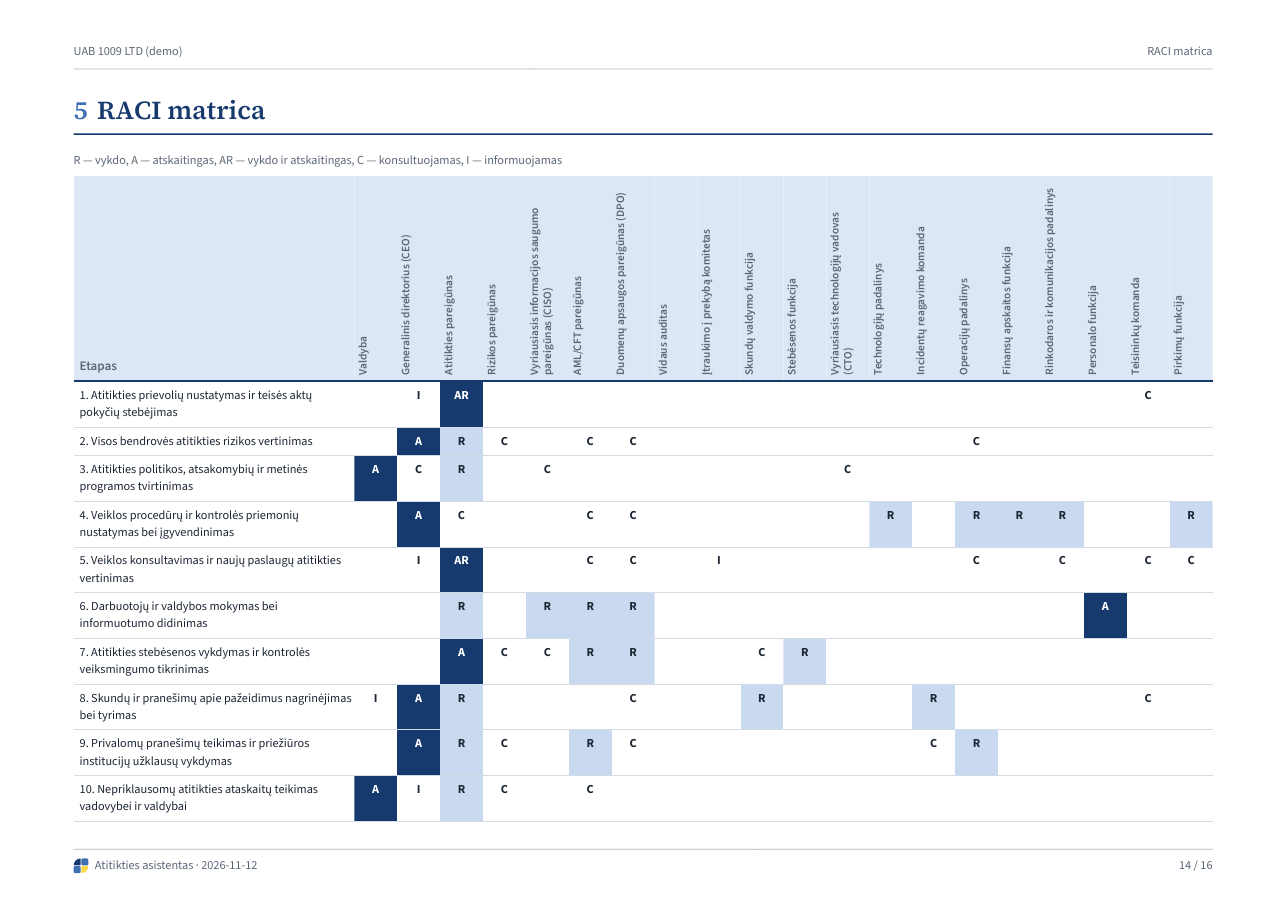
\includegraphics[width=\textwidth]{figures/samples/governance-raci}
\caption{The RACI matrix as the system's PDF export prints it for the sample company, in
Lithuanian (page 14 of 16 of a governance product generated on 12~November 2026 on a copy of
the database; a landscape page). A row per step of the process, a column per role of the
structure; A and AR in ink, R in pale blue, C and I as plain letters. The page holds the first
ten of the fourteen steps, each with exactly one A or AR.}\label{fig:programme:racipage}
\end{figure}

\subsection{The rules of a governance product}

Two groups of rules are structural and blocking: the tree and its lines of defence, and the
golden rule of the matrix. Both are counted by a few lines of \code{governance.validate}.

\begin{codebox}{The lines of defence and the golden rule, as the code has them}
A node of the second line may not report to a node of the first line. A node of the third
line that has a parent may report only to a node of the governing line. Any other placement
passes this rule; a second- or third-line node without a parent is caught by the rule
\code{structure} instead:

\begin{codeblock}
subordinated = [node["name"] for node in nodes if node["line"] == "second" and node["parentId"]
                and by_id[node["parentId"]]["line"] == "first"]
subordinated += [node["name"] for node in nodes if node["line"] == "third" and node["parentId"]
                 and by_id[node["parentId"]]["line"] != "governing"]
\end{codeblock}

For the matrix, \code{cells} maps a step and a role to one value. A letter is counted wherever
it occurs in a value, so \code{AR} counts once as accountable and once as responsible:

\begin{codeblock}
letters = lambda step_id, letter: sum(letter in value for (cell_step, _), value in cells.items() if cell_step == step_id)
accountable = [step["name"] for step in steps if letters(step["id"], "A") != 1]
responsible = [step["name"] for step in steps if letters(step["id"], "R") < 1]
\end{codeblock}

A step is listed under \code{raci_accountable} when it has no accountable role or more than
one, and under \code{raci_responsible} when nobody does the work. A process without steps
breaks both rules.
\end{codebox}

\begin{xltabular}{\textwidth}{@{}L{34mm}L{17mm}Y@{}}
\caption{The rules \code{governance.validate} checks, in the order it reports them}\label{tab:programme:govrules}\\
\toprule
\hd{Rule} & \hd{Effect} & \hd{Kept when} \\
\midrule
\endfirsthead
\toprule
\hd{Rule} & \hd{Effect} & \hd{Kept when} \\
\midrule
\endhead
\bottomrule
\endlastfoot
\code{structure} & blocking & The structure has at least one node; every node without a parent is on the governing line or on the external one, and at least one of them on the governing line; and no node names a parent that is not a node. \\
\code{independence} & blocking & No second-line node is under a first-line node, and no third-line node is under a node that is not on the governing line. \\
\code{process} & blocking & The process has at least \code{MIN_STEPS}~=~5 steps. \\
\code{raci_accountable} & blocking & There are steps, and every step has exactly one role whose value contains A. \\
\code{raci_responsible} & blocking & There are steps, and every step has at least one role whose value contains R. \\
\code{raci_everywhere} & warning & No role holds a letter in every step. \\
\code{raci_heavy} & warning & No role is accountable in more than half of the steps. \\
\code{process_basis} & warning & Every step has at least one basis entry that names a known clause or paragraph. \\
\code{quotes} & warning & Every quotation of every position stands in the document it names. \\
\end{xltabular}

Before the rules are checked the structure is made a forest by construction: a node whose
parent is not a node, is itself, or would close a circle loses its parent and becomes a top
node. The rule \code{structure} then asks that some top node be a governing body and that
nothing else hang nowhere: on top stands a governing body, an outside party --- an auditor, a
supervisor --- may stand beside the tree, and every other node has its place under one. A
node that named a parent which is not a node, and a top node on any line but the governing
and the external one, are listed by name in the rule's detail (\code{detached} in
\code{governance.validate}), so that a unit the model left unconnected is seen before the
chart is approved, where it would be drawn as a second top of the organisation. For
\code{process_basis} the code knows which references exist: the set \code{ISO_CLAUSES} holds
the 41 clause numbers of ISO~37301:2021 from 4.1 to 10.2, and a paragraph of the guidelines
is known when its number lies between 1 and 79 (\code{GUIDELINE_PARAGRAPHS}). A reference
outside both is kept in the content; a step none of whose references is known is named in the
detail of the warning.

The two matrix warnings repeat what the prompt says in words: a role with a letter in every
step is doing too much or is listed out of habit, and a role accountable for most steps is a
bottleneck. They are warnings because a small firm may have no alternative; the reviewer
decides.


% ------------------------------------------------------------
\section{Legal risk: criteria, scenarios and the register}\label{sec:programme:risks}

The risk product (\file{programme/risks.py}) follows the method of ISO~31022 on the management
of legal risk as the course teaches it: criteria first, then scenarios scored against them on
a 5×5 matrix. The division of labour is strict. The model words the criteria and writes and
scores the scenarios on eight dimensions. The code owns everything that is a number or a
fixed scale: the names of the levels, the bands and the responses each allows, the
likelihood, the impact, the score, the band and the ids.

\subsection{The criteria and the bands}

The criteria are two tables of five levels by four dimensions (\cref{tab:programme:criteria}).
The level names and the dimension keys are constants; the model fills the forty cells, each a
phrase of six to twenty words that lets a level be recognised.

\begin{table}[H]
\caption{The two sides of the criteria (\code{LIKELIHOOD}, \code{IMPACT} and their dimensions)}\label{tab:programme:criteria}
\begin{tabularx}{\textwidth}{@{}L{20mm}L{48mm}Y@{}}
\toprule
\hd{Side} & \hd{Levels 1 to 5} & \hd{Dimensions} \\
\midrule
Likelihood & Very unlikely, Unlikely, Possible, Likely, Almost certain &
  \code{control} --- internal control and competence; \code{clarity} --- legal clarity and
  supervisory practice; \code{counterparty} --- reliability of counterparties and third
  parties; \code{frequency} --- frequency and probability over time \\
Impact & Insignificant, Minor, Moderate, Major, Catastrophic &
  \code{financial} --- financial impact; \code{regulatory} --- legal, supervisory and licence
  impact; \code{reputation} --- reputation and intangible assets; \code{reach} --- reach,
  scale and domino effects \\
\bottomrule
\end{tabularx}
\end{table}

The prompt \prompt{programme.risk_criteria} gives an anchor for every dimension --- for
\code{frequency}, \code{regulatory}, \code{reputation} and \code{reach} a wording for each of
the five levels --- and opens with the test the criteria must pass:

\begin{promptexcerpt}{programme.risk_criteria}{what makes criteria usable}
[…]
The criteria will be used to score risk scenarios on a 5×5 matrix (likelihood × impact), and the governing body approves them: they must be concrete enough that two people scoring the same risk arrive at the same level.
\end{promptexcerpt}

Money is where generic criteria fail a small firm, so the financial dimension is told to
scale itself and to say what it assumed:

\begin{promptexcerpt}{programme.risk_criteria}{the financial scale}
- financial – the direct loss, fine or cost. Scale it to THIS company, not to a bank: give each level as a share of the company's annual income (or of its own funds) and, only when the profile states the turnover, also in euros. When the turnover is not stated, give the shares, add a euro range a company of this size and licence class would plausibly use, mark it as an assumption in `calibration`, and say it must be replaced once the figure is known.
\end{promptexcerpt}

The same call writes the \term{appetite}: for each of the five bands, what a risk in the band
means for this company and who decides on it. The bands themselves are not asked of the
model. The constant \code{BANDS} holds their score ranges, their names and the responses each
allows; the call is shown them under \enquote{THE BANDS OF THE MATRIX (fixed)}, and
\code{validate} rebuilds the appetite band by band from the constant, taking from the answer
only the two texts.

\begin{table}[H]
\caption{The bands of the matrix (\code{BANDS})}\label{tab:programme:bands}
\begin{tabularx}{\textwidth}{@{}L{24mm}L{16mm}L{44mm}Y@{}}
\toprule
\hd{Band} & \hd{Score} & \hd{Name} & \hd{Responses the band allows} \\
\midrule
\code{negligible} & 1--3 & Negligible (\lt{Nereikšminga}) & accept, increase \\
\code{tolerable} & 4--6 & Tolerable (\lt{Toleruotina}) & accept, mitigate \\
\code{medium} & 8--12 & Medium (\lt{Vidutinė}) & mitigate, transfer \\
\code{high} & 15--16 & High (\lt{Didelė}) & mitigate, avoid \\
\code{critical} & 20--25 & Critical (\lt{Kritinė}) & avoid \\
\bottomrule
\end{tabularx}
\end{table}

\begin{pathcard}{Legal risk criteria and appetite}{programme.risk_criteria}
  \pcrow{Trigger}{The step \code{criteria} of the job \code{programme.generate} for a product
    of kind \code{risks}.}
  \pcrow{Input}{The shared block. The data: the company's scale (size category, employees,
    annual turnover in euros, or \enquote{not stated}); the five bands with their ranges,
    names and allowed responses, from \code{BANDS}; the report brief with one example a
    theme.}
  \pcrow{Prompt and model}{\prompt{programme.risk_criteria}, version~1, on
    \model{gpt-6.1-sol} at temperature~0.2. Schema \code{CRITERIA_SCHEMA}, named
    \code{risk_criteria}. A patient call.}
  \pcrow{Output}{\code{likelihood[]}: \code{level} (1--5), \code{control}, \code{clarity},
    \code{counterparty}, \code{frequency}. \code{impact[]}: \code{level}, \code{financial},
    \code{regulatory}, \code{reputation}, \code{reach}. \code{appetite[]}: \code{band}
    (\code{negligible}, \code{tolerable}, \code{medium}, \code{high}, \code{critical}),
    \code{comment}, \code{decision}. \code{calibration}.}
  \pcrow{Checked by code}{Both tables rebuilt for the levels 1 to 5 with the level names from
    the code, each cell cut to 500 characters. The appetite rebuilt from \code{BANDS}: range,
    name and responses are the code's, only \code{comment} and \code{decision} are the
    model's; a decision is kept to 1,000 characters and the calibration to 4,000
    (\code{DECISION_CHARS}, \code{CALIBRATION_CHARS}). A blank cell, a band without its
    comment or its decision, or a missing calibration breaks the blocking rule
    \code{criteria}.}
  \pcrow{Stored}{\code{work_products.content} (\code{criteria} with \code{likelihood},
    \code{impact} and \code{calibration}; \code{appetite}).}
  \pcrow{On failure}{No retry; the product becomes \code{failed}.}
  \pcrow{Cost}{The user who started the run. Measured on 12~November 2026 on \demo{}: \$0.35
    to \$0.48 for the whole risk product, both calls.}
  \pcrow{Human control}{A person rewords any cell, the note on calibration and each band's
    meaning and decision; the bands, their ranges and their responses cannot be edited.}
  \pcrow{Measured by}{Nothing measures the prompt itself.}
\end{pathcard}

\subsection{The scenarios}

A \term{scenario} is one legal risk of the company, stated as one sentence in a fixed form
and surrounded by what a register records about it. The second call receives the criteria as
the first call worded them, four typologies, the units of the governance structure (or the
instruction to use the units the documents name), the library as refs and titles, and the
gravest open findings of the latest report. The prompt \prompt{programme.risk_scenarios}
fixes the sentence:

\begin{promptexcerpt}{programme.risk_scenarios}{the sentence every scenario follows}
THE SENTENCE
Each scenario is ONE sentence of four parts, in this form:
- in Lithuanian: "Tikėtinas [rizikos įvykis], kylantis iš [rizikos šaltinio], gali sukelti [pasekmes], kurios paveiks [saugomą tikslą]." – adjust the endings so the sentence is correct ("Tikėtina", "kylanti", "pasekmę, kuri paveiks"), but keep the four parts in this order and the words that join them ("Tikėtin…", "kylan…", "gali sukelti", "paveiks");
- in English: "A likely [risk event], arising from [risk source], may cause [consequences] that will affect [protected objective]."
\end{promptexcerpt}

The four parts --- event, source, consequences, objective --- are also returned as four
fields, so that code can tell whether one is missing. Every scenario names one or two of the
six types of legal risk of ISO~31022 Annex~A (\cref{tab:programme:types}) and one value from
each of three further typologies held in the code: six types of source (from regulators and
legislators to internal processes and IT), five of consequence, five of protected objective.
They are the lecture's typologies, and the register prints them in the lecture's words: under
a scenario's types of legal risk the card, the PDF and the workbook name its type of source,
of consequences and of protected objective (\lt{Šaltinio rūšis}, \lt{Pasekmių rūšis},
\lt{Saugomo tikslo rūšis}; \code{TYPOLOGIES} in \file{programme/exports.py} and in the
console's \file{pages/Programme/programmeUtils.js}).

\begin{table}[H]
\caption{The types of legal risk (\code{CATEGORIES}), with the words the prompt explains each in}\label{tab:programme:types}
\begin{tabularx}{\textwidth}{@{}rL{58mm}Y@{}}
\toprule
 & \hd{Type} & \hd{In the prompt's words} \\
\midrule
1 & Unpredictability of the legal environment & the law changes or is unclear \\
2 & Non-compliance with applicable laws & the company does not comply with a law that binds it \\
3 & Breach of contract & the company or its counterparty breaches a contract \\
4 & Infringement of rights & the company infringes someone's rights (clients, data subjects, holders of intellectual property) \\
5 & Omission in exercising rights & the company fails to use a right it has (to claim, to terminate, to enforce, to insure) \\
6 & Improper choice & the company makes a legally poor choice (a structure, a counterparty, a jurisdiction, a clause) \\
\bottomrule
\end{tabularx}
\end{table}

Around the sentence the model writes the area of activity and the unit that owns the risk;
the refs of one to three documents of the library the scenario concerns; the legal basis; an
\term{internal conclusion} --- what the company's documents and its latest report show about
the risk today; a level from 1 to 5 on each of the eight dimensions with a reason for each
side; a response; two to four actions; one or two owners; and a deadline as a quarter. The
prompt asks for six to ten scenarios over at least five of the six types; the rules below
require five scenarios over four, a margin left on purpose. On scoring the prompt is explicit about what the model must
not do:

\begin{promptexcerpt}{programme.risk_scenarios}{how to score, and what not to compute}
[…]
Score the impact of the reasonably foreseeable serious case – what would follow if the event happened as the scenario describes and the supervisor or the injured party acted on it – neither the mildest outcome nor the theoretical maximum, and say in `why` which case you scored.
[…]
Score what the input shows, not what would make a tidy matrix: a risk whose control is documented and tested is low on control however grave its impact, and not every risk of a regulated firm is high. Do not compute a total: the register takes the likelihood as the rounded mean of its four levels, the impact as the highest of its four, and their product as the score.
\end{promptexcerpt}

\Cref{fig:programme:registerpage} shows two scenarios of a real register with everything
around the sentence.

\begin{figure}[H]
\centering
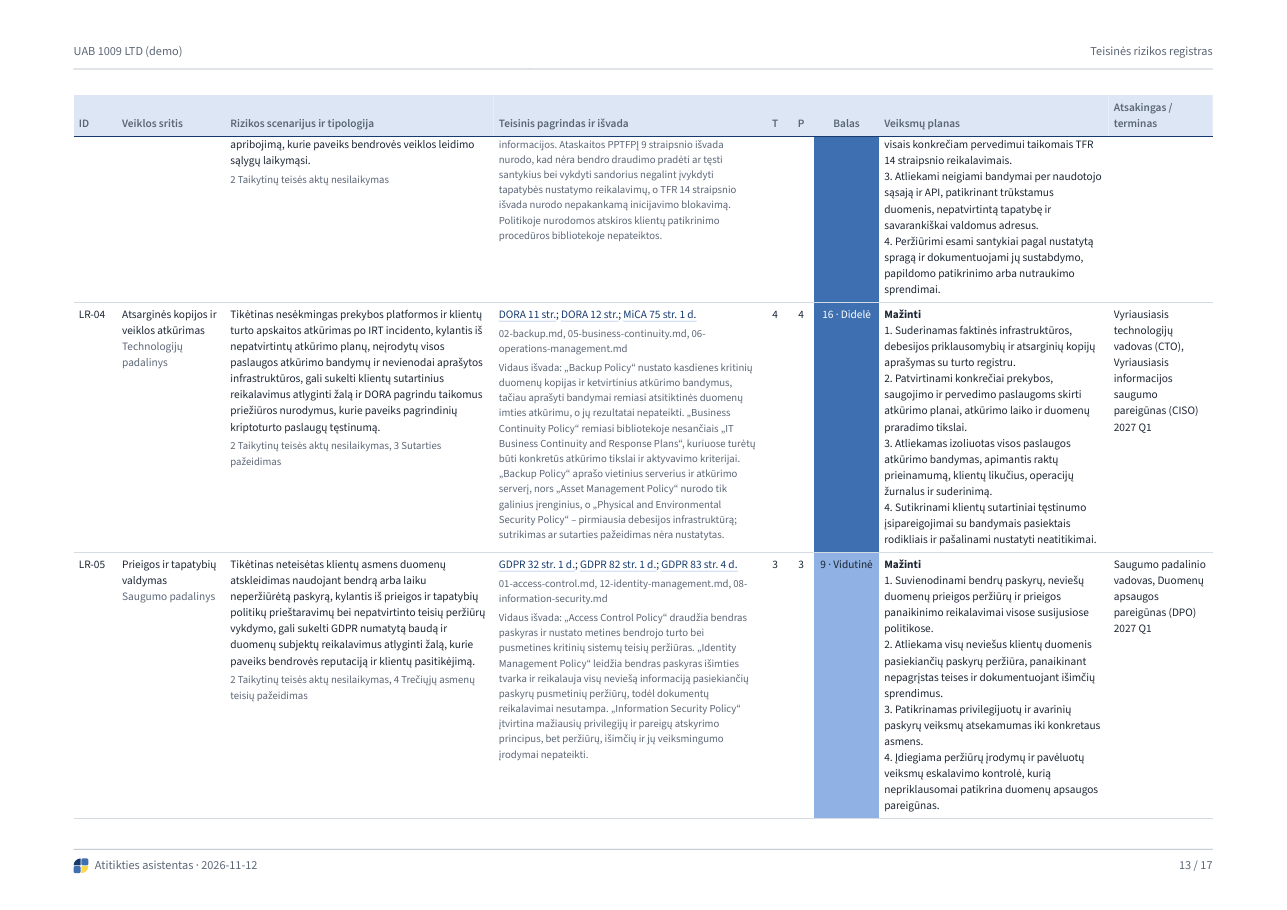
\includegraphics[width=\textwidth]{figures/samples/risks-register}
\caption{The legal risk register as the system's PDF export prints it for the sample company,
in Lithuanian (page 13 of 17 of a risk product generated on 12~November 2026 on a copy of the
database; a landscape page): the end of one scenario and two whole ones. Per row: the id; the
area of activity and the unit that owns the risk; the scenario's sentence with its types of
legal risk; the legal basis, the documents it concerns and the internal conclusion
(\lt{Vidaus išvada}); the likelihood $T$, the impact $P$, and the score with its band, which
the code computes; the response with its actions; the owners and the quarter.}\label{fig:programme:registerpage}
\end{figure}

\subsection{Numbers are computed, never taken from the model}

The schema of the scenarios has no field for a likelihood level, an impact level, a score or
a band. If an edited content carries such values, \code{validate} overwrites them. The
arithmetic is five lines.

% The box opens with a block of code, which cannot be split: room for both
\needspace{15\baselineskip}
\begin{codebox}{The arithmetic of a scenario (\code{risks.validate}, \code{band_of})}
\begin{codeblock}
level = lambda value: value if isinstance(value, int) and not isinstance(value, bool) and 1 <= value <= 5 else 0

chance = {dimension: level((row.get("likelihood") or {}).get(dimension)) for dimension in LIKELIHOOD_DIMENSIONS}
harm = {dimension: level((row.get("impact") or {}).get(dimension)) for dimension in IMPACT_DIMENSIONS}
scored = all(chance.values()) and all(harm.values())
# The likelihood is the mean of its dimensions, halves up; the impact the gravest of its dimensions
t = int(sum(chance.values()) / len(chance) + 0.5) if scored else 0
p = max(harm.values()) if scored else 0
band = band_of(t * p) if scored else None
\end{codeblock}

\begin{codeblock}
def band_of(score):
    for band, (_, highest, *_rest) in BANDS.items():
        if score <= highest:
            return band
    return "critical"
\end{codeblock}

\begin{itemize}
  \item \textbf{Likelihood} $T$: the mean of the four likelihood levels, a half rounded up.
  \item \textbf{Impact} $P$: the highest of the four impact levels. One catastrophic
        consequence is a catastrophic impact, whatever the other three are.
  \item \textbf{Score}: $T \times P$. \textbf{Band}: the first band of
        \cref{tab:programme:bands} whose upper bound the score does not exceed.
  \item \textbf{Id}: the scenario's position in the list, as \code{LR-01}, \code{LR-02}, …,
        numbered anew on every save.
  \item A level that is not a whole number from 1 to 5 counts as not set. A scenario with
        any level not set has $T = P = 0$, the score 0 and no band, and breaks the rule
        \code{scores}.
\end{itemize}

Example, from the module's test: likelihood levels 3, 2, 2, 3 have the mean 2.5, so $T = 3$;
impact levels 2, 4, 3, 2 give $P = 4$; the score is 12 and the band \code{medium}.
\end{codebox}

\begin{figure}[H]
\centering
\begin{tikzpicture}[x=14mm, y=9.5mm]
  \foreach \l in {1,...,5} {
    \foreach \p in {1,...,5} {
      \pgfmathtruncatemacro{\programmescore}{\l*\p}
      \ifnum\programmescore<4 \def\programmefill{tint}\def\programmetext{body}%
      \else\ifnum\programmescore<7 \def\programmefill{pale!45}\def\programmetext{body}%
      \else\ifnum\programmescore<13 \def\programmefill{pale}\def\programmetext{body}%
      \else\ifnum\programmescore<17 \def\programmefill{mid}\def\programmetext{white}%
      \else \def\programmefill{ink}\def\programmetext{white}%
      \fi\fi\fi\fi
      \path[fill=\programmefill, rounded corners=1.5pt] (\l-0.46,\p-0.44) rectangle (\l+0.46,\p+0.44);
      \node[text=\programmetext, font=\sffamily\small\bfseries] at (\l,\p) {\programmescore};
    }
  }
  \draw[ink, line width=1.3pt, rounded corners=1.5pt] (3-0.46,4-0.44) rectangle (3+0.46,4+0.44);
  \foreach \l/\name in {1/Very unlikely, 2/Unlikely, 3/Possible, 4/Likely, 5/Almost certain}
    \node[font=\sffamily\scriptsize, text=muted, text width=13mm, align=center, anchor=north] at (\l,0.5) {\textbf{\l}\\ \name};
  \foreach \p/\name in {1/Insignificant, 2/Minor, 3/Moderate, 4/Major, 5/Catastrophic}
    \node[font=\sffamily\scriptsize, text=muted, anchor=east] at (0.45,\p) {\name\enspace\textbf{\p}};
  \node[font=\sffamily\scriptsize\bfseries, text=mid, anchor=north] at (3,-0.55) {LIKELIHOOD $T$ (mean of four dimensions, rounded)};
  \node[font=\sffamily\scriptsize\bfseries, text=mid, anchor=south, rotate=90] at (-1.45,3) {IMPACT $P$ (highest of four)};
  \foreach \i/\fillc/\name/\range in {5/ink/Critical/20--25, 4/mid/High/15--16, 3/pale/Medium/8--12, 2/pale!45/Tolerable/4--6, 1/tint/Negligible/1--3} {
    \path[fill=\fillc, rounded corners=1.5pt] (6.0,\i-0.25) rectangle (6.45,\i+0.25);
    \node[font=\sffamily\scriptsize, anchor=west] at (6.55,\i) {\textbf{\name}\enspace\range};
  }
\end{tikzpicture}
\caption{The 5×5 matrix and its five bands. Each cell shows the score its two levels give. The
products of two levels from 1 to 5 never fall between the bands' ranges. The outlined cell is
the example of the text: $T = 3$, $P = 4$, score 12.}\label{fig:programme:matrix}
\end{figure}

The console obeys the same rule. The scenario form sends only the eight levels and
\enquote{never puts a number where a person has not chosen one}
(\file{pages/Programme/ScenarioEditor.jsx}); a scenario whose levels were edited and not yet
saved shows no level and is left out of the matrix until the server has answered. The chat
assistant is told to quote the register's numbers and never to recompute or re-band them
(\cref{sec:programme:chat}). One input the scores do not have is stated here as a known
limitation: the sanction tiers the system reads from the acts (\cref{ch:obligations}) do not
feed the impact levels, which remain the model's reading of the criteria.

\begin{figure}[H]
\centering
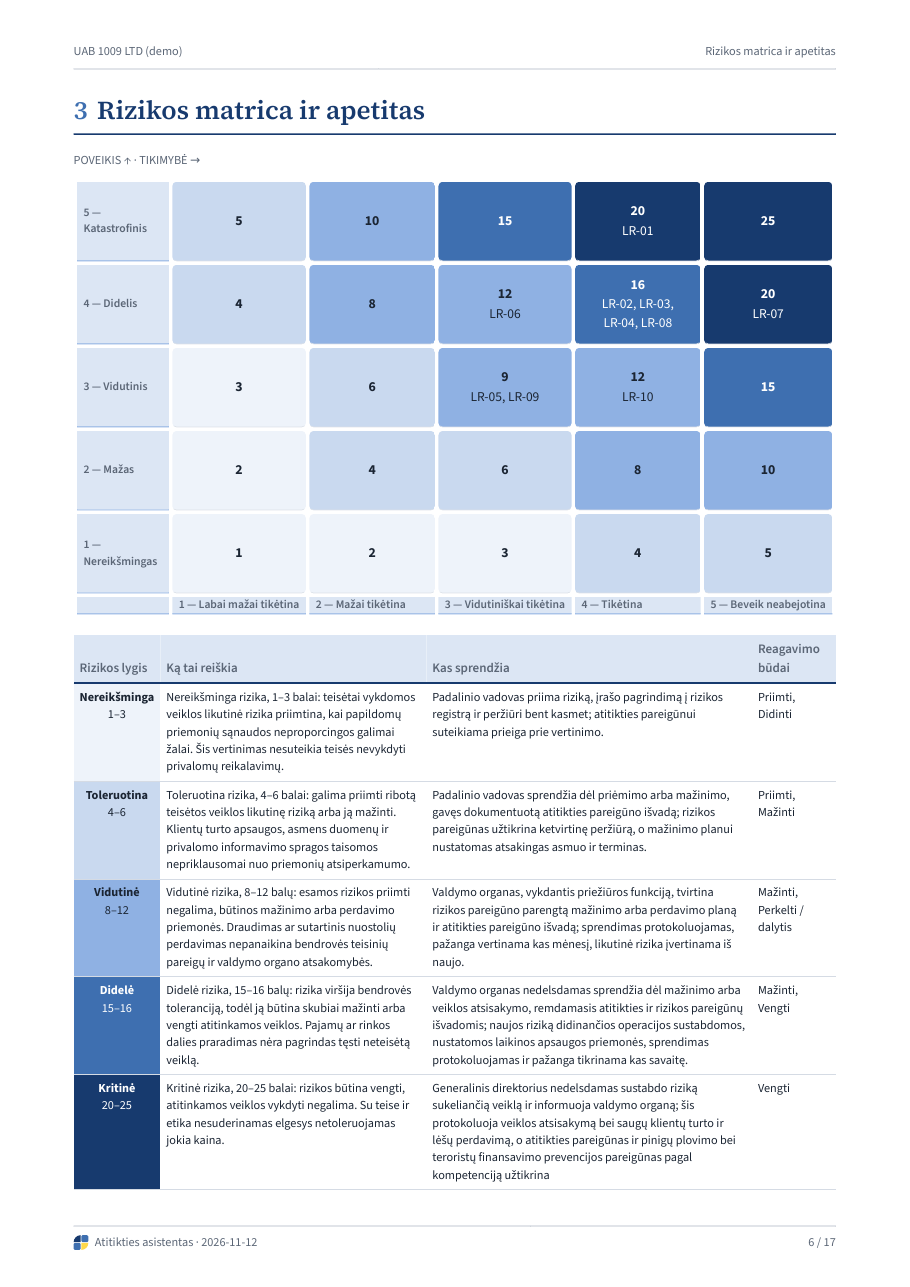
\includegraphics[width=.6\textwidth]{figures/samples/risks-matrix}
\caption{The matrix of the same register as its PDF export prints it (page 6 of 17, in
Lithuanian): impact upwards, likelihood to the right, each cell with its score and the ids of
the scenarios that fall in it --- of the ten, two in the critical band, four high and four
medium. Below, the five bands of the product's criteria, with what each means, who decides and
the responses it allows.}\label{fig:programme:matrixpage}
\end{figure}

\subsection{The rules of a register}

\begin{xltabular}{\textwidth}{@{}L{37mm}L{17mm}Y@{}}
\caption{The rules \code{risks.validate} checks, in the order it reports them}\label{tab:programme:riskrules}\\
\toprule
\hd{Rule} & \hd{Effect} & \hd{Kept when} \\
\midrule
\endfirsthead
\toprule
\hd{Rule} & \hd{Effect} & \hd{Kept when} \\
\midrule
\endhead
\bottomrule
\endlastfoot
\code{criteria} & blocking & None of the forty cells of the two criteria tables is blank, every band of the appetite has its comment and its decision, and the calibration is written. The detail is the number of blanks. \\
\code{scenarios} & blocking & There are at least \code{MIN_SCENARIOS}~=~5 scenarios. \\
\code{categories} & blocking & The scenarios together name at least \code{MIN_CATEGORIES}~=~4 of the six types of legal risk. \\
\code{sentence} & blocking & Every scenario has its sentence and all four of its parts: event, source, consequences, objective. \\
\code{ties} & blocking & Every scenario names a unit and at least one policy that is a document of the company. \\
\code{scores} & blocking & Every scenario has all eight levels as whole numbers from 1 to 5. \\
\code{provisions} & blocking & No provision named by a scenario has the status \code{not_found}. \\
\code{provisions_unverified} & warning & No provision names an act the corpus does not hold. \\
\code{provision_subjects} & warning & No provision was judged \code{mismatch}. \\
\code{owners} & warning & Every scenario has at least one owner and a deadline. \\
\code{response_fit} & warning & Every scored scenario's response is one its band allows. \\
\code{sentence_form} & warning & Every sentence contains, ignoring case, the four joining words of its language: \enquote{Tikėtin}, \enquote{kylan}, \enquote{gali sukelti}, \enquote{paveik} in Lithuanian; \enquote{likely}, \enquote{arising from}, \enquote{may cause}, \enquote{affect} in English. \\
\end{xltabular}

Normalisation does the rest: a scenario keeps at most two types, the two lowest numbers it
names; a response outside the five becomes \code{mitigate}; a policy that is no document of the company is dropped, which is how
an invented ref ends as a broken \code{ties} rule. One field has no counterpart in the
schema: \code{externalConclusion}, the view of an outside lawyer, which only a person can
write on the scenario's form. And one field has no check at all: the internal conclusion is
the model's free text about the company, tied to its sources only by the instruction to use
facts from the input. It is the part of a scenario a reviewer should read first.

\begin{pathcard}{Legal risk scenarios}{programme.risk_scenarios}
  \pcrow{Trigger}{The step \code{scenarios} of the same job, directly after the step
    \code{criteria}.}
  \pcrow{Input}{The same shared block. The data: the two criteria tables as the first call
    wrote them; the types of legal risk and the typologies of sources, consequences and
    objectives; the names of the governance structure's nodes of kind \code{unit} or
    \code{function}, or a note that there is no structure product; the library as refs and
    titles; up to 36 open findings of the latest report, gravest first, 220 characters of
    analysis each.}
  \pcrow{Prompt and model}{\prompt{programme.risk_scenarios}, version~1, on
    \model{gpt-6.1-sol} at temperature~0.3. Schema \code{SCENARIOS_SCHEMA}, named
    \code{risk_scenarios}. A patient call.}
  \pcrow{Output}{\code{title}; \code{scenarios[]}: \code{area}, \code{unit},
    \code{sentence}, \code{event}, \code{source}, \code{consequences}, \code{objective},
    \code{categories[]} (1--6), \code{sourceType} (1--6), \code{consequenceType} (1--5),
    \code{objectiveType} (1--5), \code{legalBasis[]}, \code{policyRefs[]},
    \code{internalConclusion}, \code{likelihood} (four levels 1--5 and \code{why}),
    \code{impact} (four levels 1--5 and \code{why}), \code{response} (\code{accept},
    \code{increase}, \code{mitigate}, \code{transfer}, \code{avoid}), \code{actions[]},
    \code{owners[]}, \code{deadline}.}
  \pcrow{Checked by code}{Ids assigned; likelihood, impact, score and band computed; policy
    refs turned into the company's documents; provisions looked up and judged once; the
    twelve rules of \cref{tab:programme:riskrules}.}
  \pcrow{Stored}{\code{work_products.content} (\code{title}, \code{scenarios}).}
  \pcrow{On failure}{No retry; the criteria of the first call are lost with the run.}
  \pcrow{Cost}{The user who started the run; part of the \$0.35 to \$0.48 measured for the
    product.}
  \pcrow{Human control}{A person edits a scenario's fields, the eight levels and its place
    in the three typologies included, adds or removes
    scenarios, may write the outside lawyer's conclusion, and approves the
    register. The levels the model gave are a draft for the reviewer to correct.}
  \pcrow{Measured by}{Nothing measures the prompt itself. Two defects seen in its first
    registers led to the changes described below.}
\end{pathcard}

\subsection{Two lessons from the first registers}

The scenarios prompt reached its present wording through two observations on the sample
company, recorded in \file{docs/markdown/en/architecture.md}. Neither fault is one a rule of the kind can
detect: no rule looks at how the scores spread or at which policies the scenarios concern.

\begin{lessonbox}{12 November 2026: flat impact scores}
The first register generated for \demo{} gave nine of its ten scenarios the same impact
levels --- \enquote{a fine, the licence not presumed lost} --- and placed a doubt about the
scope of the authorisation itself nowhere. The prompt was changed to tell the model to weigh
each scenario on its own facts and to put first the risks that could cost the company its
authorisation, its clients' assets or the continuity of a core service. The second register
spread its scores from 9 to 20. (The prompt also tells the model to score the reasonably
foreseeable serious case and to say which case it scored; see the excerpt above.)
\end{lessonbox}

\begin{lessonbox}{12 November 2026: scenarios leaning on the financial policies}
The second register tied its scenarios to the financial policies alone, where the course's
assignment ties scenarios to the technology, operations and security units and their
policies. The prompt now says so in words:

\begin{promptexcerpt}{programme.risk_scenarios}{cover the organisation}
[…]
Cover the organisation, not one corner of it: where the company has units for technology, for operations and for security, each of them owns at least one scenario, and at least a third of the scenarios turn on its operational and information-security policies (access control, backup, business continuity, operations, assets, incidents, suppliers) – legal risk arises there too: a contract breached when a restore fails, personal data lost through access nobody reviewed, a right against a supplier never used.
\end{promptexcerpt}

The third register had ten scenarios over all six types of legal risk and six units, with
seven of the information-technology policies among the seventeen documents they concern.
\end{lessonbox}


% ------------------------------------------------------------
\section{A person's turn: editing, approval, new versions}\label{sec:programme:person}

A generated product is a draft on its own page in the console
(\file{pages/Programme/ProductPage.jsx}). Above the content stands the panel \ui{Taisyklės}
(Rules): a sentence saying how many blocking rules are broken, or that none is, and every rule
of the kind with its state --- \ui{laikomasi} (kept), \ui{pažeista} (broken) or \ui{pastaba}
(note) --- and the detail of what broke it. Below it the content is shown in the tabs of the
kind (\cref{tab:programme:tabs}); the last tab of every kind, \ui{Kilmė} (Provenance), lists
what the run read, the prompt versions and models behind it, and its cost.

\begin{table}[H]
\caption{The tabs of a product's page and what a person can change in a draft}\label{tab:programme:tabs}
\begin{tabularx}{\textwidth}{@{}L{20mm}L{38mm}Y@{}}
\toprule
\hd{Kind} & \hd{Tab} & \hd{Editable in a draft} \\
\midrule
\code{policy} & \ui{Politika} (Policy) & Each part's text, its decisions and its legal basis; the headings are fixed. \\
 & \ui{Dokumentai} (Documents) & Each document's level and topic; each missing document's title, purpose, level, priority and provisions, or its removal. \\
\code{governance} & \ui{Struktūra} (Structure) & The nodes: name, kind, line, parent, the proposed flag, the note; nodes added and removed. \\
 & \ui{Procesas ir RACI} (Process and RACI) & The steps with their basis; every cell of the matrix; a role added as a column. \\
 & \ui{Pareigybės ir spragos} (Positions and gaps) & Nothing: a record of what the generation found. \\
\code{risks} & \ui{Registras} (Register) & A scenario's fields, the eight levels included, but not its source, consequence and objective types; scenarios added and removed. \\
 & \ui{Kriterijai} (Criteria) & The wording of every cell, the calibration note, each band's meaning and decision. \\
\bottomrule
\end{tabularx}
\end{table}

\subsection{An edit goes through the same validation}

\ui{Redaguoti} (Edit) turns the content into forms. The edits stay in the page until the
person saves them; the save sends the whole content with
\route{PUT}{/api/programme/{id}/content}. The view \code{product_content} refuses anything
but a draft (409 \code{NOT_DRAFT}) and calls the same \code{validate} that the generation
called, without the \code{judge} argument, which means without a model: quotes are located
again, provisions looked up again, levels, scores, bands and ids computed again, and every
rule checked again. What it stores, and answers, is the normalised content with its new
checks, the editor's name and the time. The page replaces its own copy with the answer, so
what is on screen after a save is what the server holds, with any rule the edit mended or
broke.

The consequence is that a person and a model are held to the same rules by the same code. A
person can mend a draft --- remove a provision the act does not have, give a step its
accountable role --- and a person can break one: an edit that leaves a step with two
accountable roles makes the draft unapprovable until it is corrected.

\subsection{Approval freezes a product}

\ui{Patvirtinti} (Approve) opens a dialog that says what approval means and takes an optional
note. The request is
\route{PATCH}{/api/programme/{id}} with \code{approved: true}. The view \code{product_item}
accepts it only for a draft, and only when no check that is blocking is broken; otherwise it
answers 409 \code{RULES_BROKEN} and names the rules. The page disables the button in
advance, with the reason, while a blocking rule is broken or the draft has unsaved edits. An
approval records who approved, when, and the note (at most 2,000 characters), and is audited
as \code{programme.approve}. Any user who may see the company --- its owner or an
administrator --- may approve; the chat assistant has no tool that does.

An approved product cannot be edited: \code{PUT} refuses it. \ui{Nauja versija} (New version)
sends \route{POST}{/api/programme/{id}/revise}, which copies the approved content and its
checks into a new draft with the next version number and \code{revisedFrom} in its basis; the
approved version stays as it was approved. The route refuses when a newer version of the kind
is already queued, running or a draft (409 \code{NEWER_VERSION}). A revised draft has no run
of its own, so its provenance shows no prompts and no cost.

\begin{figure}[H]
\centering
\begin{tikzpicture}[node distance=15mm and 19mm]
  \node[svc, minimum width=19mm] (queued) {queued};
  \node[ai, minimum width=19mm, right=of queued] (running) {running};
  \node[chk, minimum width=19mm, right=of running] (draft) {draft\\ {\scriptsize version $n$}};
  \node[man, minimum width=19mm, right=of draft] (approved) {approved\\ {\scriptsize frozen}};
  \node[svc, minimum width=19mm, below=of queued] (cancelled) {cancelled};
  \node[svc, minimum width=19mm, below=of running] (failed) {failed};
  \node[chk, minimum width=19mm, below=of approved] (next) {draft\\ {\scriptsize version $n{+}1$}};
  \draw[flow] (queued) -- node[lbl, above, align=center] {the worker\\ takes the job} (running);
  \draw[flow] (running) -- node[lbl, above, align=center] {the rules\\ are checked} (draft);
  \draw[flow] (draft) -- node[lbl, above, align=center] {a person\\ approves} node[lbl, below, align=center] {no blocking\\ rule broken} (approved);
  \draw[flow] (queued) -- node[lbl, left, align=right] {a person\\ stops it} (cancelled);
  \draw[flow] (running) -- (cancelled);
  \draw[flow] (running) -- node[lbl, right, align=left] {an error, or\\ the worker died} (failed);
  \draw[flow] (approved) -- node[lbl, left, align=right] {a person revises:\\ a copy} (next);
  \draw[flow] (draft.south west) .. controls +(-5mm,-9mm) and +(5mm,-9mm) .. node[lbl, below, align=center] {a person saves an edit:\\ validated again, no model} (draft.south east);
\end{tikzpicture}
\actorlegend
\caption{The states of one version of a work product. The colour of a state says who
produces it: model calls run while it is \code{running}, code has checked a \code{draft}, and
only a person makes it \code{approved}. A version in any state but \code{queued} and
\code{running} can be deleted.}\label{fig:programme:states}
\end{figure}

\subsection{Stopping and deleting}

\ui{Stabdyti generavimą} (Stop the generation) sends \route{POST}{/api/programme/{id}/cancel}.
A queued job is cancelled at once; a running one is flagged and stops before its next model
call, so a call already under way is finished and paid for. A version that is not queued or
running can be deleted with \route{DELETE}{/api/programme/{id}} --- an approved one too; the
other versions stay. Creating, editing, approving, revising, cancelling, deleting and
exporting a product each write an audit entry (\cref{ch:security}).


% ------------------------------------------------------------
\section{The structure chart and the exports}\label{sec:programme:outputs}

\subsection{One drawing for the page and the paper}

The structure of a governance product is drawn by the API, not by the console:
\code{structure_svg} in \file{programme/chart.py} turns the nodes into one SVG image, served
by \route{GET}{/api/programme/{id}/chart} for the page and embedded in the PDF. The page and
the paper therefore cannot differ. The console fetches the image as a file and shows it in an
image element; the SVG markup is never inserted into the page, and every text in it is
escaped.

Each node is a box under its parent, 180 by 66 units, with the name on at most three lines of
23 characters. The box is coloured by its line --- the governing bodies in the brand's ink,
the first line pale, the second outlined in blue, the third marked in yellow, external
assurance grey --- and drawn with a dashed outline and the word \lt{siūloma} (proposed) when
the node is proposed. A legend under the tree repeats the colours in words. The layout is
that of an organisation chart: the upper levels spread as rows, the children of a node
ordered by line so that the three lines read from left to right; children that have nothing
under them do not take a column each but hang together, up to five on one rail
(\code{RAIL}); deeper levels are stacked under their parent, indented a step per level. How
many levels spread as rows --- one, two or three --- is whichever makes the drawing best fit a
landscape page's box of 263 by 148 (\code{PAGE_W}, \code{PAGE_H}).

\begin{figure}[H]
\centering
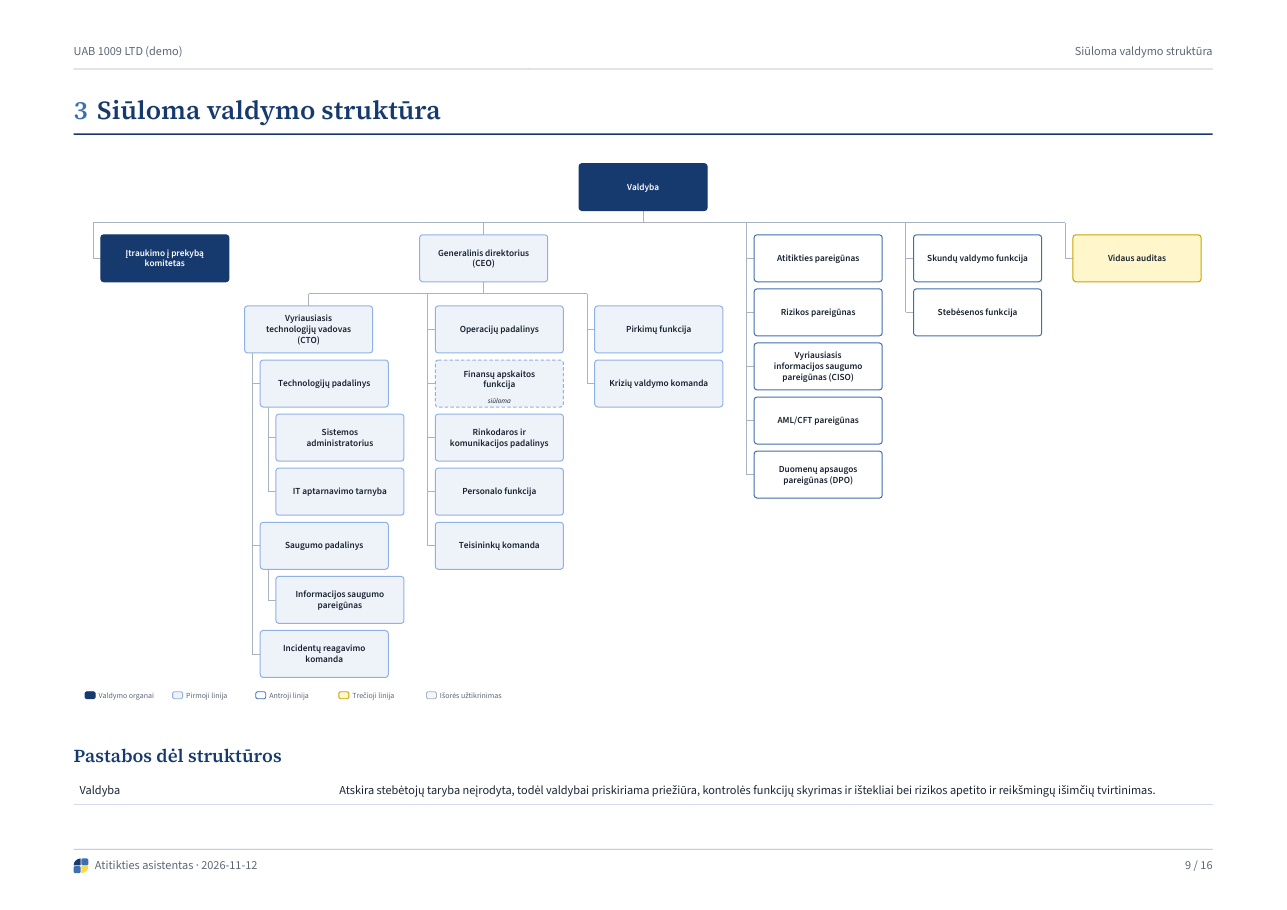
\includegraphics[width=\textwidth]{figures/samples/governance-chart}
\caption{The proposed structure as the PDF export prints it (page 9 of 16 of the governance
product of \cref{fig:programme:racipage}; a landscape page): the same image the console
shows. The governing bodies in ink --- the board (\lt{Valdyba}) and a committee; the first line
in pale boxes under the chief executive; the second line outlined in blue; internal audit, the
third line, in yellow; the finance function, which the model proposes, dashed and marked
\lt{siūloma}; the legend under the tree. Below it begin the notes on the structure.}\label{fig:programme:chartpage}
\end{figure}

\subsection{The exports}

\route{GET}{/api/programme/{id}/export?format=} hands a draft or an approved product over as a
file (\file{programme/exports.py}); a product in any other state has nothing to export.

\begin{table}[H]
\caption{The export formats of each kind (\code{FORMATS})}\label{tab:programme:exports}
\begin{tabularx}{\textwidth}{@{}L{20mm}L{13mm}Y@{}}
\toprule
\hd{Kind} & \hd{Format} & \hd{What the file holds} \\
\midrule
all & PDF & A cover; the contents; the product in numbered sections; a last section, \enquote{Checks and provenance}, with every rule as the product met or broke it and what it was made from. \\
\code{policy} & Word & The title, the company, the version and whether it is a draft; the eight parts under numbered headings; the points left to the governing body gathered at the end. \\
\code{risks} & Excel & Four sheets: the register in fourteen columns, the likelihood criteria, the impact criteria, and the bands with their meaning, decision and responses. \\
\bottomrule
\end{tabularx}
\end{table}

The PDF is made with the report's stylesheet, fonts and page furniture
(\file{analysis/pdf.py}, \cref{ch:report}), so a company's report and its programme read as
one set. Its cover states the kind, the title, the company, the date and the version, and
either who approved the product and when or \enquote{Draft --- not yet approved by a person}.
The policy's sections are its eight parts --- each with the open decisions in a callout, the
documents it rests on and its legal basis as links to the official text --- followed by the
hierarchy and the missing documents, each with the part of the policy it serves. The governance PDF sets the chart and the RACI matrix on
landscape pages, the matrix with the role names running up their columns and the accountable
cell filled in ink. The risk PDF gives the two criteria tables, the matrix with every
scenario's id in the cell its levels put it in, followed by the table of bands, the scenarios
one by one --- each with its types of legal risk and its place in the three typologies ---
and the register on a landscape page in nine columns.

The two other formats exist because of what is done with the documents next. A board edits a
policy before adopting it, hence a Word file; a register is kept and worked with, hence a
workbook. In the workbook every cell is stored as text or a number, so no text of a product
can become a formula.


% ------------------------------------------------------------
\section{What the chat can and cannot do}\label{sec:programme:chat}

The chat assistant (\cref{ch:chat}) reaches work products through two tools, defined in the
assistant service in \file{llm/tools/programme.js} and listed with all others in
\cref{app:tools}.

\begin{table}[H]
\caption{The chat's two tools for work products}\label{tab:programme:chat}
\begin{tabularx}{\textwidth}{@{}L{34mm}Y@{}}
\toprule
\hd{Tool} & \hd{What it does} \\
\midrule
\code{startWorkProduct} & Calls the same route as the console's button, with the kind and a language. A refusal of the API --- no documents, one already running, the budget spent --- comes back as an answer that says what to do next, not as an error. \\
\code{getWorkProduct} & With the company alone: the newest version of every kind and its status. With a kind or a product id: that product, rebuilt small. With \code{section}: only the criteria tables of a register, or only the positions of a governance product. \\
\bottomrule
\end{tabularx}
\end{table}

A product's content is some 80~kB as the API keeps it, and it is never passed to the model
whole. \code{getWorkProduct} rebuilds it: a provision becomes one string with a mark where the
lookup warns, a quotation becomes the title of its document, the structure an indented
outline, the matrix one line a step with the roles by name. The rules the product does not
keep come in words, the blocking ones apart from the notes. Every answer about a product
carries the address of the product's page.

The chat cannot edit a product and cannot approve one; no tool exists for either. The prompt
\prompt{chat.assistant} draws the line in its rule on work products:

\begin{promptexcerpt}{chat.assistant}{rule 12, on work products}
[…]
When there is none, offer to generate it: it works in the background for about five minutes and takes about 0.5 USD of today's budget – startWorkProduct only after the user's yes, the policy first, then the structure, then the register, since each builds on the ones before it. While one is being generated say so and go on. Never write such a document yourself in the chat in place of the product, and never call one approved: only a person approves, on its page.
\end{promptexcerpt}

The reason for the last sentence is the difference this chapter is about. A policy the chat
wrote into a conversation would have passed no rule, would rest on no located quotation and no
looked-up provision, and would have no version and no approver.


% ------------------------------------------------------------
\section{Cost and measurements}\label{sec:programme:cost}

All six prompts run on \model{gpt-6.1-sol}, which the gateway's price list of 10~November 2026
puts at \$2 per million input tokens, \$10 per million output tokens, \$0.10 for input read
from the cache and \$2.50 for input written to it. A run is two calls over the same library:
the first writes the shared block to the provider's cache and the second reads it from there
(\cref{ch:models}).

The budget is checked once, at the start: the user needs \$0.25 left for the day. A run that
has started is not stopped by the daily budget. The two calls of the kind and any inventory
are recorded against the user who started the job. The citation judge's call in the
\code{references} step is recorded under the job step without a user: it is part of the cost
the product shows on its provenance tab, which sums every call of the job, but not of
anyone's daily budget. The console tells the user before starting that a run takes about five
minutes and about \$0.50 (\code{RUN_COST_USD} in \file{pages/Companies/CompanyProgramme.jsx});
the chat's tool description says four to six minutes.

\begin{lessonbox}{Measured, 12 November 2026}
One product of each kind was generated for \demo{} on a copy of the database, on
\model{gpt-6.1-sol} (\file{docs/markdown/en/architecture.md}):

\begin{tabularx}{\linewidth}{@{}L{24mm}L{22mm}Y@{}}
\toprule
\hd{Kind} & \hd{Cost} & \hd{What came out} \\
\midrule
\code{policy} & \$0.46, five minutes & Eight parts; 23 of 23 quotations located; 24 of 24 provisions found; 16 missing documents. \\
\code{governance} & \$0.39 & 46 positions, 15 gaps, 25 nodes, 14 steps; the golden rule kept; one warning --- the compliance officer takes part in every step. \\
\code{risks} & \$0.35 to \$0.48 & Ten scenarios over all six types of legal risk and six units; every rule kept. \\
\bottomrule
\end{tabularx}

\smallskip
These are runs on one company on one day. They show that the rules can be met, not how
often they are.

On the live system on 13~November 2026 one product of each kind was generated again for
\demo{}: the policy for \$0.51 in five minutes, every rule kept; the structure, process and
RACI for \$0.53 in six and a half minutes, fourteen steps, every rule kept; the register for
\$0.49 in five and a half minutes, ten scenarios over five of the six types of legal risk,
with two warnings that do not block approval --- a legal basis in the Civil Code, which the
corpus does not hold, and one MiCA provision the citation judge found to regulate something
else. All three are drafts: no person has approved them.
\end{lessonbox}


% ------------------------------------------------------------
\section{How it is known to work}\label{sec:programme:evaluation}

No evaluation suite measures these six prompts. The suites the system has
(\cref{ch:control}) cover the judge of the register, the scope reading, the citation judge,
the gap analysis, applicability and sanctions; none generates a work product and compares it
with an expected one. The quality of a draft is held in two other ways.

\begin{description}
  \item[By code, to the rules.] Every draft, whoever wrote it, passes through
    \code{validate}. The rules establish that a product is complete, that its structure and
    its matrix are well formed, that its numbers follow from its levels, and that its
    references exist. \file{tests/test_programme.py} tests this code with a stand-in model:
    that a policy comes out a draft with its rules checked, that a person can mend, approve
    and revise it, that the golden rule and the independence of the lines are enforced, that
    no level, score or band is taken on trust, that every possible score falls in a band, and
    that the exports and the chart are produced. These tests say nothing about what the real
    model writes.
  \item[By a person, to judgement.] Whether the policy fits the company, whether a role is
    really missing, whether a RACI assignment is sensible, whether a scenario's internal
    conclusion is true and its levels are right --- no rule decides any of this. The person
    who approves the product decides it, and the system records who that was.
\end{description}

The two lessons of \cref{sec:programme:risks} show why the second matters: neither fault was
one a rule could catch. Until a suite of reference products exists, an approved work
product is as reliable as its reviewer's reading of it; a draft is a starting point, and the
cover of every PDF says which of the two the reader is holding.

Two further limits belong here. The system does not produce the annual compliance report or a
monitoring programme: the three kinds are the whole of what it drafts. And a library larger
than 600,000 characters cannot be given a work product at all, since the run refuses to work
from excerpts (\cref{sec:programme:library}).
